\documentclass[11pt]{article}
\usepackage{graphicx}
\usepackage[margin=2.5cm]{geometry}
\usepackage{tikz}
\usepackage{indentfirst}
\usepackage{tabularx}
\usepackage{listingsutf8}
\usepackage{color}
\usepackage{hyperref}
\usepackage[portuguese]{babel}

\graphicspath{{./images/}}

\def\checkmark{\tikz\fill[scale=0.4](0,.35) -- (.25,0) -- (1,.7) -- (.25,.15) -- cycle;} 
\setlength{\parskip}{0.5em}

\renewcommand{\lstlistingname}{Código}
\renewcommand{\lstlistlistingname}{Pedaços de Código}

\definecolor{dkgreen}{rgb}{0,0.6,0}
\definecolor{gray}{rgb}{0.5,0.5,0.5}
\definecolor{mauve}{rgb}{0.58,0,0.82}

\hypersetup{
	colorlinks=false,
	linktoc=all,
	hidelinks,
}

\lstset{
	belowcaptionskip=1\baselineskip,
	captionpos=b,
	frame=tb,
	language=C,
	aboveskip=3mm,
	belowskip=3mm,
	showstringspaces=false,
	columns=flexible,
	basicstyle={\small\ttfamily},
	numbers=none,
	numberstyle=\tiny\color{gray},
	keywordstyle=\color{blue},
	commentstyle=\color{dkgreen},
	stringstyle=\color{mauve},
	breaklines=true,
	breakatwhitespace=true,
	tabsize=3,
	inputencoding=utf8,
	extendedchars=true,
	literate={á}{{\'a}}1 {ã}{{\~a}}1 {à}{{\`a} }1 {Ã}{{\~A}}1 {ó}{{\'o}}1 {Ó}{{\'O}}1 {Í}{{\'I}}1 {í}{{\'i}}1 {é}{{\'e}}1 {ç}{{\c{c}}}1 {Ç}{{\c{C}}}1 {ú}{{\'u}}1 {õ}{{\~o}}1
}

\begin{document}
	\begin{titlepage}
    	\begin{center}
    		
\includegraphics[width=0.6\textwidth]{logo-isec}
    		
    		\vspace*{\fill}
    		
    		\Huge
    		\textbf{Programação Avançada}
    		
    		\huge
    		4 em Linha
    		
    		\vspace{0.5cm}
    		\LARGE
    		2020 - 2021
    		
    		\vspace{1.5cm}
    		
    		\textbf{TheForgotten}
    		
    		\vspace*{\fill}
    		
\includegraphics[width=0.2\textwidth]{logo-java}
    		
    		\vfill
    		\vspace*{\fill}
    		
    		\normalsize
    		Licenciatura de Engenharia Informática \\
    		23 de maio de 2021		
    	\end{center}
    \end{titlepage}
	
	\tableofcontents
	\pagebreak
	
	\large
	\section{Introdução}
	\normalsize
	
	O trabalho prático consiste na implementação de um jogo em Java.
	
	O jogo é o 4 em linha. Neste, dois jogadores tentam alinhar 4 das suas peças na vertical, horizontal ou diagonal. O primeiro a fazer uma linha de quatro peças ganha.
	
	O trabalho prático foi concretizado em linguagem Java e, nesta meta, acompanhado por uma interface consola. Na meta seguinte será construída uma GUI para substituir a atual CLI.
   	
	
	\large
	\section{Diagrama da Máquina de Estados}
	\normalsize
	
	\begin{figure}[h]
		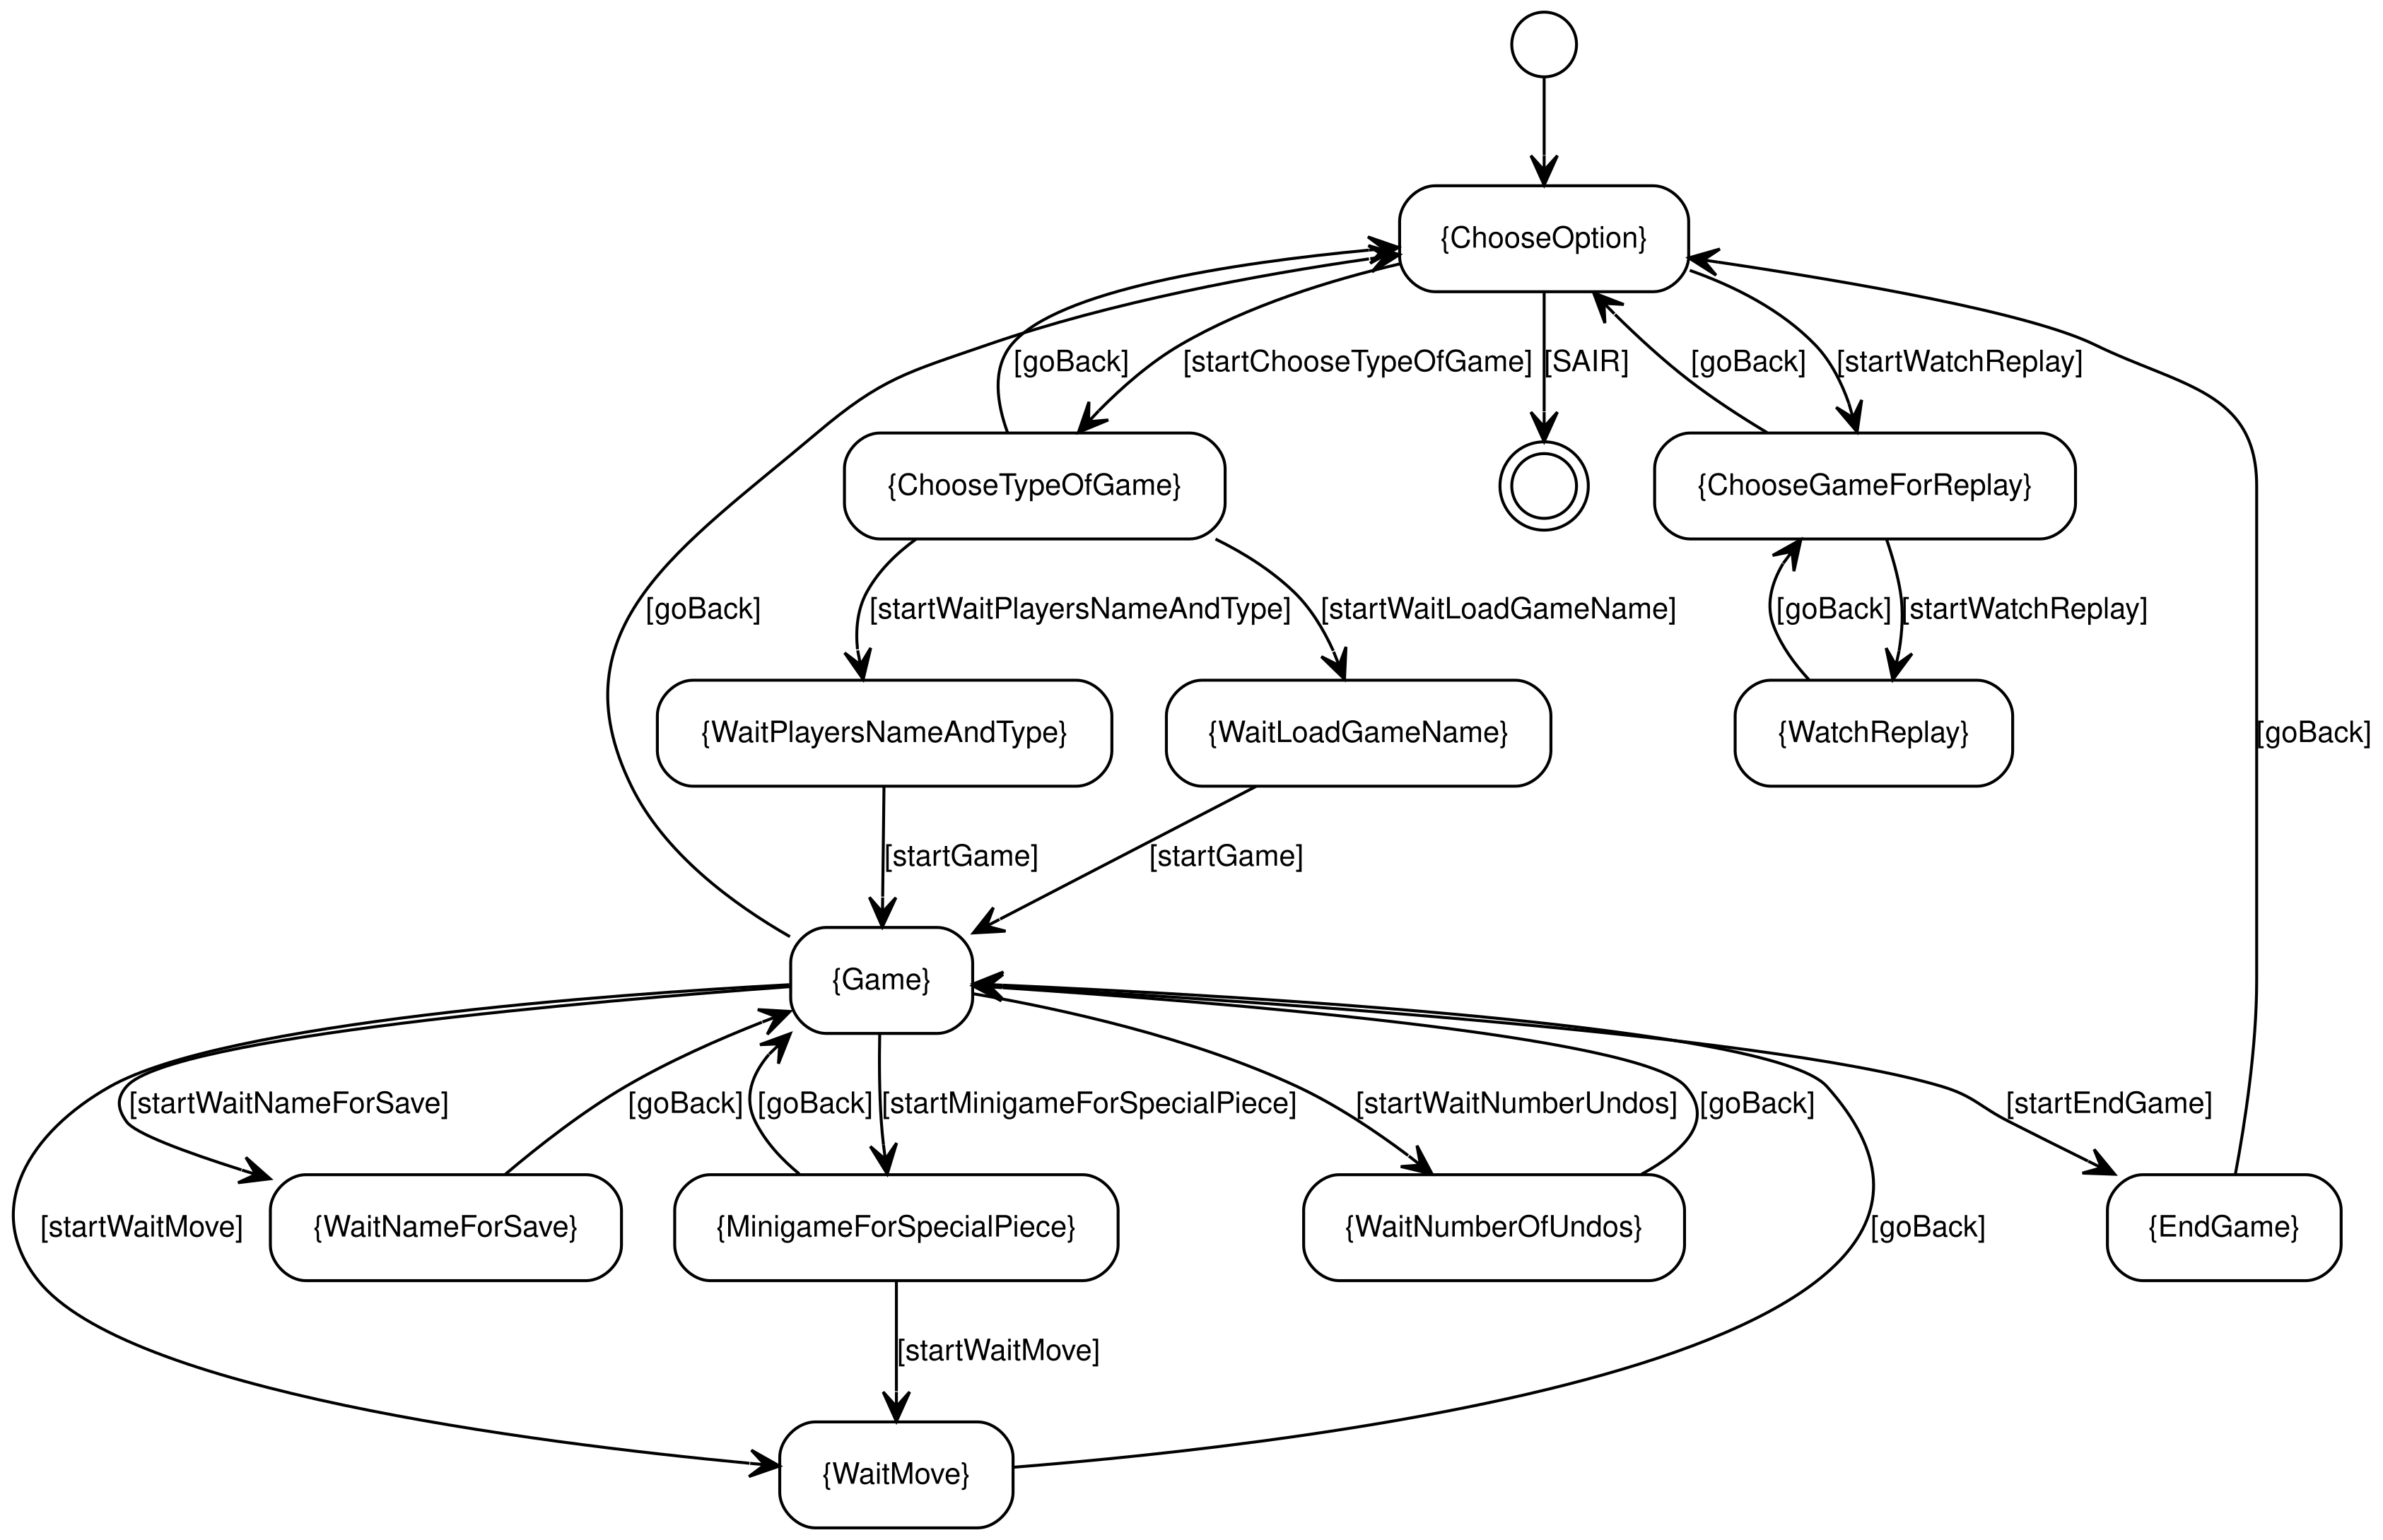
\includegraphics[width=0.95\textwidth,height=0.88\textheight,keepaspectratio]{state-machine-diagram}
		\centering
		\caption{Diagrama da Máquina de Estados}
		\label{fig:sm-diagram}
	\end{figure}
	
	Este diagrama de estados foi feito em yUML e o ficheiro código encontra-se em anexo.
	
	
	\large
	\section{Arquitetura Geral}
	\normalsize
	
	O IDE usado foi IntelliJ IDEA.
	
	Usando o paradigma de programação com máquina de estados, a classe \textbf{JogoCLI} comunica exclusivamente com a máquina de estados, que irá então depois delegar o resto da lógica. Para além disso faz recurso a alguns métodos static para tratamento de input e output de modo a manter o código mais limpo e legível.
	
	Existem duas classes utilitárias no programa, sendo uma a \textbf{UtilsUI} e a outra a \textbf{UtilsFiles}. A primeira contém vários métodos que ajudam no tratamento de input e output, a segunda contém vários métodos para ajudar na leitura e gravação de ficheiros. Estas possuem os seus métodos declarados como static.
	
	A máquina de estados trata da lógica de evolução da interface, ou seja, é com esta que evoluímos de estados mas toda a lógica envolvente ao jogo é depois delegada para uma classe chamada \textbf{JogoManager}.
	
	A classe \textbf{JogoManager} é a primeira a ter acesso direto ao jogo. Esta classe trata assim do \textbf{Jogo} e do \textbf{CommandManager}. Deste maneira, esta é responsável por decidir que métodos devem ou não fazer uso do \textbf{CommandManager}. Esta é também a classe que é gravada em ficheiro de save ou replay dum jogo.
	
	Exemplificando, se eu quiser jogar uma peça na coluna 1, a \textbf{JogoCLI} pede-me a coluna, esta coluna é enviada para a \textbf{StateMachine}, a \textbf{StateMachine} envia para o estado, o estado envia para o \textbf{JogoManager}, o \textbf{JogoManager} envia para o \textbf{CommandManager}, o \textbf{CommandManager} invoca o comando necessário, o comando invocado finalmente comunica com o \textbf{Jogo}.
	
	
	\large
	\section{Classes Usadas}
	\normalsize
	
	As principais classes usadas no programa são as que se seguem. De modo a não ter um relatório excessivamente extenso, irão apenas ser mencionadas Interfaces e Adapters.
	
	\large
	\subsection{JogoApp}
	\normalsize

	Classe que contém a main. Apenas responsável por inicializar a \textbf{StateMachine} e a \textbf{JogoCLI}.
	
	
	\large
	\subsection{JogoCLI}
	\normalsize
	
	Classe que serve de interface. É esta que interage com o utilizador. Toda a informação recebida é depois tratada pelas classes de lógica.
	
	
	\large
	\subsection{StateMachine}
	\normalsize
	
	Esta classe representa a máquina de estados. É esta que trata toda a lógica da máquina.
	
	
	\large
	\subsection{IState}
	\normalsize
	
	Classe interface dos estados. Esta é depois implementada pelo \textbf{StateAdapter}.
	
	
	\large
	\subsection{StateAdapter}
	\normalsize
	
	Classe que implementa a \textbf{IState}. Esta é depois extendida por todos os outros estados.
	
	
	\large
	\subsection{JogoManager}
	\normalsize
	
	Classe que gere o \textbf{Jogo} e o \textbf{CommandManager}. Todos os comandos para enviar ao jogo passam por aqui e esta decide se precisam de integrar o \textbf{CommandManager} ou não.
	
	
	\large
	\subsection{CommandManager}
	\normalsize
	
	Classe que gere certos comandos do jogo e guarda um histórico destes. Atinge isto com recurso a métodos que invocam comandos e fazem undo dos mesmo implementados por classes que implementam e extendem a classe interface \textbf{ICommand}.
	
	
	\large
	\subsection{ICommand}
	\normalsize
	
	Classe interface dos commandos. Esta é depois implementada pelo \textbf{CommandAdapter}.
	
	
	\large
	\subsection{CommandAdapter}
	\normalsize
	
	Classe que implementa a \textbf{ICommand}. Esta é depois extendida por todos os outros comandos.
	
	
	\large
	\subsection{Minigame}
	\normalsize
	
	Classe abstrata que possuí a lógica base para o funcionamento de um minijogo. Esta é depois extendida pelos minigames.
	
	
	\large
	\subsection{Player}
	\normalsize
	
	Classe abstrata que possuí a lógica base para o funcionamento de um jogador. Esta é depois extendida pelos players.
	
	\large
	\subsection{Jogo}
	\normalsize
	
	Esta é a classe que possuí toda a lógica do jogo.
	
	
	\large
	\subsection{UtilsUI}
	\normalsize
	
	Classe com apenas métodos estáticos. Serve para ajudar no tratamento de informação vinda do utilizador.
	
	
	\large
	\subsection{UtilsFiles}
	\normalsize
	
	Classe com apenas métodos estáticos. Serve para ajudar no tratamento de ficheiros.
	
	
	\large
	\subsection{AppStates, JogoStates \& TypePiece}
	\normalsize
	
	Para além das classes mencionadas anteriormente, o jogo possuí também 3 enumerações.
	
	\begin{itemize}
		\item \textbf{AppStates:} possui os estados da máquina de estados;
		\item \textbf{JogoStates:} possui os estados do jogo;
		\item \textbf{TypePiece:} possui os tipos de peça que o tabuleiro pode ter;
	\end{itemize}


	\large
	\section{Relacionamento Entre as Classes}
	\normalsize
	
	A interface \textbf{IState} é implementada pela classe \textbf{StateAdapter}, que por sua vez é extendida pelas classes que representam estados na máquina de estados: \textbf{ChooseGameForReplay}, \textbf{ChooseOption}, \textbf{ChooseTypeOfGame}, \textbf{EndGame}, \textbf{Game}, \textbf{MinigameForSpecialPiece}, \textbf{WaitLoadGameName}, \textbf{WaitMove}, \textbf{WaitNameForSave}, \textbf{WaitNumberOfUndos}, \textbf{WaitPlayersNameAndType} e \textbf{WatchReplay}.
	
	Os estados são geridos pela classe \textbf{StateMachine} que vai invocando métodos dos estados e mantém sempre o estado atual.
	
	A interface \textbf{ICommand} é implementada pela classe \textbf{CommandAdapter}, que por sua vez é extendida pelas classes que representam os diferentes comandos: \textbf{PlacePieceOnColumn}, \textbf{PlaceSpecialPieceOnColumn} e \textbf{UpdateJogo}.
	
	Os comandos são geridos pela classe \textbf{CommandManager} que, para além de os invocar, também os guarda para possibilitar as funcionalidades de desfazer jogada e ver replay.
	
	A classe abstrata \textbf{Minigame} é extendida pelas classes que representam os diferentes minijogos: \textbf{MathMinigame} e \textbf{TypingMinigame}.
	
	Os minijogos são geridos exclusivamente pelo estado \textbf{MinigameForSpecialPiece}.
	
	A classe abstrata \textbf{Player} é extendida pelas classes que representam os diferentes tipos de jogador: \textbf{PlayerAI} e \textbf{PlayerHuman}.
	
	Os jogadores são geridos pela classe \textbf{Jogo}.
	
	A classe \textbf{Jogo} possuí toda a lógica para o funcionamento do jogo.
	
	Esta é gerida pela classe \textbf{JogoManager}, que gere também a classe \textbf{CommandManager}. Esta é a responsável por invocar métodos do \textbf{Jogo} e decidir quais devem ser invocados pelo \textbf{CommandManager}.
	
	A introdução de dados pelo utilizador é tratada pela \textbf{JogoCLI}, que por sua vez delega essa informação para a \textbf{StateMachine}, que por sua vez a envia para o \textbf{IState} atual, que depois a envia para o \textbf{JogoManager}, que irá então escolher se precisa de usar o \textbf{CommandManager} ou se pode comunicar diretamente com o \textbf{Jogo}.
	
		
	\large
	\section{Funcionalidades Implementadas}
	\normalsize
	
	\begin{tabularx}{\textwidth}{|X|c|c|c|}
		\hline
		\textbf{Funcionalidade} & \textbf{Realizado} & \textbf{Realizado Parcialmente} & \textbf{Não Realizado} \\
		\hline
		Interface de Linha de Consola & \checkmark & & \\
		\hline
		Jogo Base 4 Em Linha & \checkmark & & \\
		\hline
		Jogador Virtual & \checkmark & & \\
		\hline
		Minijogos para Peça Especial & \checkmark & & \\
		\hline
		Desfazer Jogadas & \checkmark & & \\
		\hline
		Replay de Jogos Finalizados & \checkmark & & \\
		\hline
		Manter um Máximo de 5 Replays & \checkmark & & \\
		\hline
		Criar e Carregar Saves & \checkmark & & \\
		\hline
	\end{tabularx}

	\large
	\section{Conclusão}
	\normalsize
	
	Servindo como maneira para aprender programação com máquinas de estado e também como maneira para aplicar o paradigma de programação orientada a objetos, este trabalho foi uma excelente oportunidade não só de aprendizagem como também de reforço de conhecimentos.
	
	Para além disto, é também uma boa introdução a programação em Java, ficando assim mais familiarizado com as suas vantagens e desvantagens.
	
	
	\pagebreak
	
	\large
	\section{Anexos}
	\normalsize
	
	\listoffigures
	% \lstlistoflistings
\end{document}